\chapter{Plano de Integração}
\label{chapter:plano}

Neste capítulo apresentamos nosso planejamento para a integração dos diferentes
subsistemas, que deve ocorrer na terceira etapa do projeto. Adaptamos os pontos
levantados no guia do PMBOK, adequando o plano ao contexto da disciplina, e
focando na integração de subsistemas de um projeto de engenharia, e não da área
de gestão de pessoas.

A integração dos subsistemas ocorrerá no tempo das aulas, contudo, caso
necessário, em outros horários o grupo se reunirá de forma a conseguir a
integração completa. Ainda, ressaltamos que o subsistema de Processamento de
Sinais e Monitoramento não é fortemente acoplado aos outros subsistemas, de
modo que a integração entre ele e o restante do projeto será fácil e não
carecerá de um grande esforço. Os outros dois subsistemas, Projeto Estrutural
e Controle e Alimentação, por outro lado, são bem acoplados, e um maior cuidado
será tomado a respeito desses dois subsistemas.

\section{Integração do subsistema Processamento de Sinais e Monitoramento}

Como mencionado, o subsistema de Processamento de Sinais e Monitoramento não
deverá apresentar grandes problemas na integração, principalmente por não ser
acoplado aos outros subsistemas. Os únicos componentes físicos desse subsistema
são os componentes eletrônicos relacionados a aquisição de sinais (sensores,
amplificadores, filtros e conversores) e o sistema embarcado (Raspberry Pi).
Os outros componentes (servidor remoto, cliente \textit{frontend} e
\textit{mobile}) estão na nuvem, e não causam impacto na integração com os
outros componentes físicos.

Para o terceiro ponto de controle também faremos o desenvolvimento dos
componentes que tornem o UMISS mais tolerante a falha, através de circuitos
que adicionem redundância ao projeto. Essa tolerância ocorrerá através da
adição do módulo GPRS/3G, que possibilitará uma alternância no envio de dados
caso a \textit{internet} da residência do paciente esteja indisponível, ou
ainda em casos onde a energia da residência ou fatores externos afetem a
conexão. Outro esforço será empregado na
adição dos componentes que detectam a presença do paciente na cadeira, que
será importante em diversos cenários.  Por exemplo, caso o paciente caia da
cadeira, os sensores de temperatura podem capturar valores anômalos, que devem
ser ignorados.

É esperado que os componentes físicos desse subsistema sejam alocados em um
compartimento de fácil manutenção, para que seja facilmente manuseado durante
os diversos testes. Além disso, esse compartimento deve disponibilizar saídas
para os fios, que serão então conectados a outros subsistemas, ou
disponibilizados para serem utilizados pelo paciente. Assim, a integração deve
ocorrer da seguinte forma:

\begin{enumerate}
    \item Alocação dos componentes eletrônicos de modo seguro, mas que ocupe
        o menor espaço possível, pois os outros subsistemas carecem de bastante
        espaço;
    \item Acoplamento do compartimento na parte inferior da cadeira (nos braços),
        parafusando-o (incluindo o \textit{case} da Raspberry Pi);
    \item Extensão e disponibilização dos cabos e dos sensores, para que sejam
        facilmente utilizados pelos pacientes;
    \item Extensão da bateria conectada a Raspberry Pi, e conexão entre ela e a
        bateria do subsistema de Controle e Alimentação.
\end{enumerate}

\section{Integração do subsistema de Estruturas}

Com as etapas mencionadas anteriormente completas, o subsistema de estruturas
tem por sua única preocupação futura de desenvolver componentes físicos que
agreguem todos os equipamentos dos demais subsistemas. Sempre se preocupando
com a facilidade de manuseio durante os testes que serão feitos. Com isso, a
integração será feita da seguinte maneira e terá como objetivo ficar similar
com a Figura \ref{fig:complete_chair}, que foi criada no ambiente CAD:

\begin{enumerate}
    \item Alocação dos equipamentos eletrônicos e do RaspBerry Pi do subsistema
    de processamento de sinais e monitoramento com suas dimensões e integra-los
    a estrutura da cadeira de maneira ergonômica, se preocupando com a
    disponibilização dos cabos e sensores, de forma que o usuário tenha seus
    sinais vitais adquiridos da maneira mais confortável possível.
    \item Outra preocupação é a interface da estrutura da cadeira e todo o
    sistema de alimentação e controle dos motores, na qual ira ser feita um
    sistema de gaveta abaixo da cadeira que ira suportar a bateria de forma
    que ela seja de fácil acesso e removível para o seu carregamento de energia.
\end{enumerate}

\begin{figure}[!htb]
    \begin{center}
        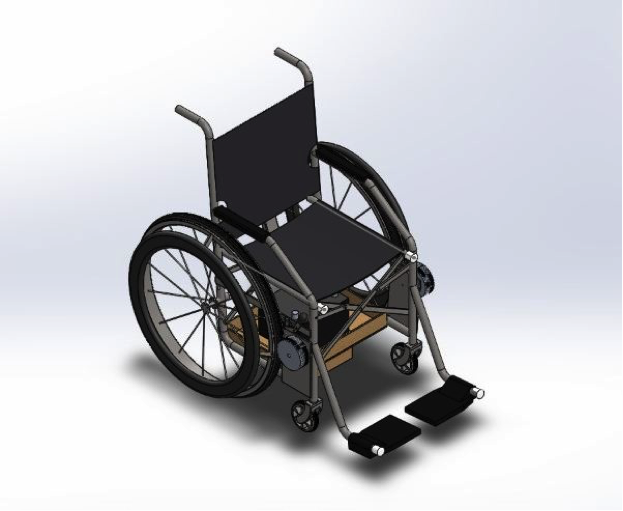
\includegraphics{figuras/complete_chair.png}
    \end{center}
    \caption{Projeto da Cadeira Completa.}
    \label{fig:complete_chair}
\end{figure}

\section{Integração do subsistema Controle e Alimentação}

O acoplamento entre o sistema Controle e Alimentação e os demais sistemas físicos se
dará através da instalação do circuito elétrico na estrutura da cadeira. O circuito deve conter
um sistema de proteção, que possa ser facilmente acessado pelo usuário em caso de
emergência, também deve ser desenvolvido um compartimento para que os circuitos dos
drivers sejam alocados de maneira que possam ser facilmente acessados para possíveis
manutenções e testes. Eles ficarão preferencialmente na parte inferior da cadeira.

A etapa de integração do sistema de alimentação demanda um maior cuidado, além de
ser de vital importância para a conclusão do projeto, dessa forma algumas atividades devem
ser bem definidas para que o projeto seja concluído com êxito. Sendo assim, a integração deve
ocorrer da seguinte forma:

\begin{enumerate}
  \item Alocação do sistema de controle dos motores (drivers), de forma acessível;
  \item Montagem do circuito de alimentação, incluindo extensão para componentes
  eletrônicos dos demais subsistemas;
  \item Realização de testes para verificação do correto funcionamento do circuito proposto.
\end{enumerate}

\section{Cronograma}

\begin{table}[!htbp]
    \centering
    \caption{Cronograma para a integração dos subsistemas.}
    \label{tab:cronogramaintegracao}
    \resizebox{\textwidth}{!}{%
        \begin{tabular}{|p{10cm}|p{6cm}|l|}
            \hline
            \textbf{Atividade} & \textbf{Responsável} & \textbf{Deadline} \\
            \hline
            Desenvolvimento do sensor de presença & Afonso & 01/06 \\
            \hline
            Criar compartimento com sensores e embarcado & Afonso, Dylan, Gustavo, Tiago e Wilton & 08/06\\
            \hline
            Acoplamento do módulo GPRS/3G aos outros componentes & Dylan e Afonso & 08/06 \\
            \hline
            Extensão e disponibilização dos cabos & Gustavo, Tiago e Wilton & 08/06 \\
            \hline
            Extensão da bateria da Raspberry Pi & Dylan e Afonso & 08/06 \\
            \hline
            Teste do subsistema de Processamento e Monitoramento & Afonso, Dylan, Gustavo, Tiago e Wilton & 08/06 \\
            \hline
            Manufatura do sistema de gaveta & Nivaldo, Rafael e Lucas Matheus & 02/06 \\
            \hline
            Acoplamento da gaveta com a bateria e eletrônicos na cadeira & Nivaldo, Rafael e Lucas Matheus & 09/06 \\
            \hline
            Criação do compartimento dos eletrônicos do processamento de sinais e monitoramento & Nivaldo, Rafael e Lucas Matheus & 16/06 \\
            \hline
            Integração da atividade acima com a estrutura da cadeira & Nivaldo, Rafael e Lucas Matheus & 23/06 \\
            \hline
            Desenvolver compartimento para alocação do sistema de controle dos motores & Mariana, Lunara, Cesar, Felipe e Johnson & 08/06 \\
            \hline
            Montagem do circuito de alimentação adaptado à estrutura da cadeira & Mariana, Lunara, Cesar, Felipe e Johnson & 08/06 \\
            \hline
            Teste do subsistema de Controle e Alimentação após integração aos demais subsistemas & Mariana, Lunara, Cesar, Felipe e Johnson & 08/06 \\
            \hline

        \end{tabular}
    }
\end{table}
